\section{Symulacje i testy}
W tym rozdziale przedstawione zostaną gramatyki renderujące różne
przedmioty oraz metody ich tworzenia. W kolejnych podrozdziałach zostaną one
dokładnie opisane. Po zaznajomieniu się z metodologią tworzenia gramatyk
zaprezentowane zostaną poszczególne elementy głowy, następnie połączone zostaną
w jedną całość.

\subsection{Proste obiekty}
Do przetestowania gramatyk kształtów wybraliśmy dwa obiekty, które mają
dosyć prostą strukturę ale jednocześnie pozwalają na wykorzystanie większości
dostępnych możliwości programu..
\subsubsection{Kostka do gry}
Pierwszym elementem poddanym analizie jest kostka do gry. Jest to element dość
prosty do zamodelowania, ponieważ można go wykonać z jednego sześcianu (ang.
cube) i 21 kul, którymi zostaną wycięte otwory oznaczające ilość oczek na
konkretnej ściance kostki. Aby zadanie nieco utrudnić, dodana zostanie możliwość
wygładzania krawędzi kostki, oraz dwa parametry określające stopień wygładzenia
krawędzi i wielkość kostki.

Poniżej znajduje się kod tworzący kostkę oraz wygenerowana za pomocą aplikacji
kostka:
\begin{figure}[h!]
  \centering
  \subfloat[border = 0.1, size = 0.8]{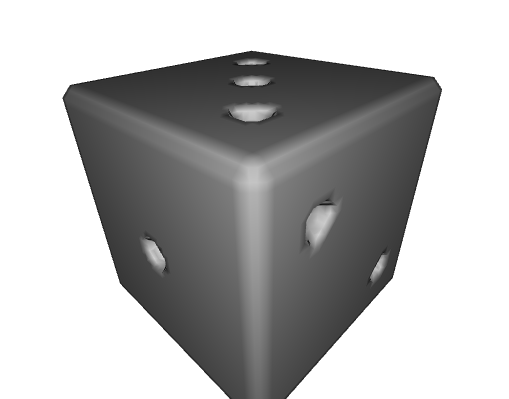
\includegraphics[width=0.4\textwidth]{images/tests/kostka01.png}}
  \qquad
  \subfloat[border = 0.5, size = 0.6]{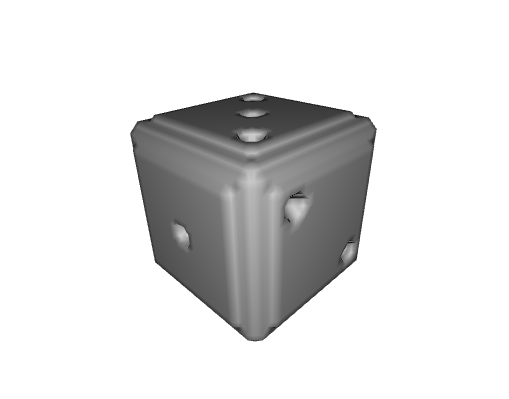
\includegraphics[width=0.4\textwidth]{images/tests/kostka02.png}}
  \caption{Kostka do gry (źródło własne).}
\end{figure}
{
\small
\begin{lstlisting}[numbers=left,frame=single,numberstyle=\tiny,backgroundcolor=\color{code_back},breaklines=true]
local border = params:getParamFloat("border");
local size   = params:getParamFloat("size");

local b = Cube();
local c1 = Cylinder();
local c2 = Cylinder();
local c3 = Cylinder();
b:scale(0.8, 0.8, 0.8);

c1:scale(1.1-border*0.2, 1.1-border*0.2, 1.1-border*0.2);
c2:scale(1.1-border*0.2, 1.1-border*0.2, 1.1-border*0.2);
c3:scale(1.1-border*0.2, 1.1-border*0.2, 1.1-border*0.2);

c2:rotateDeg(90, 0, 0);
c3:rotateDeg(0, 0, 90);

local box = And(b, c1, c2, c3);

local p1 = Sphere();
local p2 = Sphere();
local p3 = Sphere();
local p4 = Sphere();
local p5 = Sphere();
local p6 = Sphere();

p1:scale(0.1, 0.1, 0.1);
p2:scale(0.1, 0.1, 0.1);
p3:scale(0.1, 0.1, 0.1);
p4:scale(0.1, 0.1, 0.1);
p5:scale(0.1, 0.1, 0.1);
p6:scale(0.1, 0.1, 0.1);

p1:translate(0, 0, 8);

p2:translate(8, 4, 4);
p3:translate(8,-4,-4);

p4:translate(0, 8, 0);
p5:translate(4, 8, 4);
p6:translate(-4,8,-4);

local cube1 = Diff(box, p1, p2, p3);
local cube = Diff(cube1, p4, p5, p6);

cube:scale(size, size, size);

draw(cube);
/*EOS*/
border;2;0.1
size;2;0.8
\end{lstlisting}
}

W linii 1 pobierana jest wartość parametru określającego stopień wygładzenia
krawędzi kostki - dostępny przedział to $<0; 1>$, w linii 2 natomiast parametr
określający wielkość kostki i również z przedziału $<0; 1>$. Następnie w linii
3 tworzymy sześcian (ang. cube), który będzie podstawową formą kostki, oraz trzy
cylindry (linie 4-6) potrzebne do wygładzenia krawędzi --- jeden cylinder do
krawędzi równoległych po osi $Y$, drugi po $Z$ a trzeci po $X$. Kolejne linie
skalują sześcian tak, aby był on widoczny w oknie. Skalowaniu poddane zostają
też cylindry wygładzające krawędzie zgodnie z parametrem {\em border}. Linie 14
i 15 obracają cylindry tak, aby były równoległe odpowiednio z osią $Z$ i $X$.
Następnie operacją logiczną {\em And} wygładzone zostają krawędzie kostki. Kolejny etap to
utworzenie kul reprezentujących oczka kostki, aby nie rozwlekać zbytnio kodu ograniczyliśmy się
tylko do sześciu oczek, trzech widocznych ścian kostki (ściana z jednym
oczkiem, dwoma i trzema). Każde oczko skalujemy do odpowiedniego rozmiaru
(linie 26-31), kule zostają spozycjonowane w odpowiednie miejsca (linie 33-40),
aż w końcu operacją {\em Diff} zostają wycięte oczka w kostce (linie 42-43). Na
końcu kostka zostaje przeskalowana do żądanej wielkości, zgodnej z parametrem
{\em size}, oraz wyświetlona funkcją \emph{draw}.

\subsubsection{Kubek do kawy}
Drugim zamodelowanym obiektem będzie kubek. Jako parametry dla gramatyki dodane
zostanie wypełnienie kubka oraz rozmiar uchwytu dla kubka.

\begin{figure}[h!]
  \centering
  \subfloat[depth = 1.0, size = 1.0]{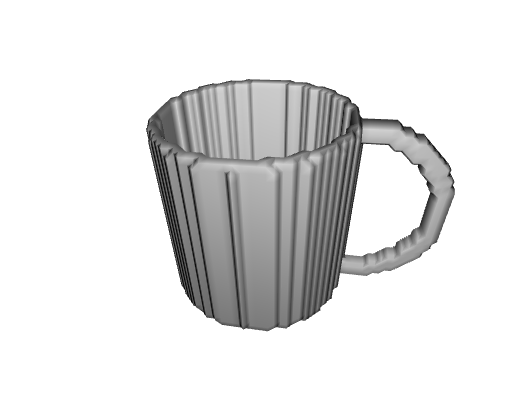
\includegraphics[width=0.4\textwidth]{images/tests/kubek01.png}}
  \qquad
  \subfloat[depth = 0.2, size = 0.8]{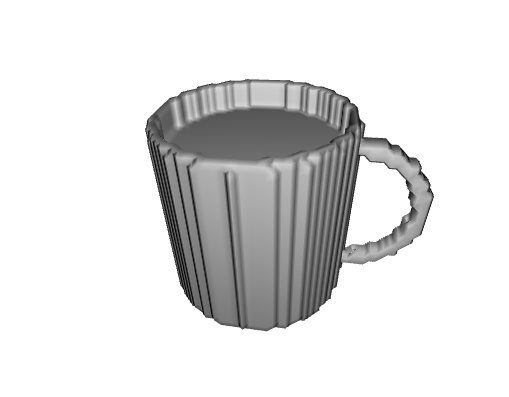
\includegraphics[width=0.4\textwidth]{images/tests/kubek02.png}}
  \caption{Kubek do kawy (źródło własne).}
\end{figure}
{
\small
\begin{lstlisting}[numbers=left,frame=single,numberstyle=\tiny,backgroundcolor=\color{code_back},breaklines=true]
local dParam = params:getParamFloat("depth");
local sParam = params:getParamFloat("size");

local cup = Cylinder();
cup:scale(0.5, 0.5, 0.5);

local cupff = Cylinder();
cupff:translate(0, 1.05 - dParam, 0);
cupff:scale(0.45, 0.5, 0.45);

local all = Diff(cup, cupff);

local round = Sphere();
round:scale(0.7, 0.7, 0.7);
all = And(all, round);

local h1 = Sphere();
h1:scale(0.5, 0.5, 0.5);
local h2 = Sphere();
h2:scale(0.4, 0.4, 0.4);
local handle = Diff(h1, h2);

local handleCut = Cube();
handleCut:scale(1, 1, 0.05);
handleCut:translate(1, 0, 0);
handle = And(handle, handleCut);
handle:translate(0.5, 0, 0);

handle:scale(sParam, sParam, sParam);

all = Or(handle, all);

draw(all);
/*EOS*/
depth;2;1
size;2;1
\end{lstlisting}
}

Na początku wczytane zostają parametry zewnętrzne {\em depth} -- wypełnienie
kubka oraz {\em size} -- rozmiar uchwytu kubka. W liniach 4-5 utworzony zostaje
kształt będący zewnętrzną częścią kubka, a w liniach 7-9 kształt stanowiący
wewnętrzną część kubka. Operacją {\em Diff} wycięte zostaje wnętrze kubka.
W liniach 13-14 przygotowywany jest kształt do zaokrąglenia górnych i dolnych
krawędzi kubka a następnie w linii 15 jest on nakładany na obiekt. W kolejnych
dziesięciu liniach jest przygotowywany kształt uchwytu do kubka -- dwoma kulami
wycięta zostaje cienka sfera, a następnie prostopadłościanem jest przycięta do
wąskiego paska. W 29 linii skalowany jest jeszcze uchwyt do rozmiaru podanego
jako parametr, aż w końcu w linii 31 uchwyt zostaje połączony do kubka i za
pomocą funkcji {\em draw} (linia 33) kubek zostaje wyświetlony na ekranie.

\subsection{Głowa ludzka}
Znając już metodę tworzenia obiektów w programie można przejść do zamodelowania
głowy ludzkiej. Proces został podzielony na cztery etapy:
\begin{itemize}
  \item przygotowanie gramatyki oczu;
  \item przygotowanie gramatyki nosa;
  \item przygotowanie gramatyki ust;
  \item przygotowanie gramatyki uszu;
  \item przygotowanie gramatyki pozostałej części głowy oraz dołożenie elementów
  przygotowanych wcześniej.
\end{itemize}

\subsubsection{Gramatyka oka}
Najprostszym obiektem do zamodelowania okazało się oko, głównie ze względu na
to, że jest ono bardzo podobne do sfery. Jako parametry wybrana została pozycja
gałki ocznej (lewo-prawo) -- {\em eye\_lr} i poziom otwartych powiek -- {\em eye\_open}.

\begin{figure}[h!]
  \centering
  \subfloat[eye\_lr = 0.0, eye\_open = 1.0]{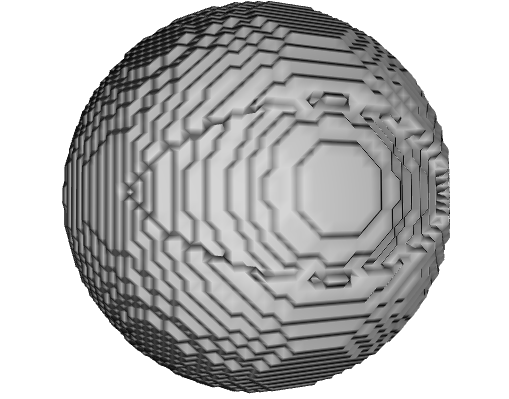
\includegraphics[width=0.4\textwidth]{images/tests/eye01.png}}
  \qquad
  \subfloat[eye\_lr = 0.0, eye\_open = 0.5]{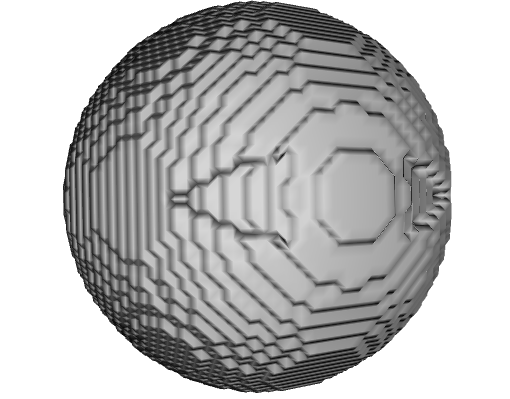
\includegraphics[width=0.4\textwidth]{images/tests/eye02.png}}
  \caption{Wyrenderowane oko (źródło własne).}
\end{figure}

\begin{figure}[h!]
  \centering
  \subfloat[eye\_lr = 0.7, eye\_open = 1.0]{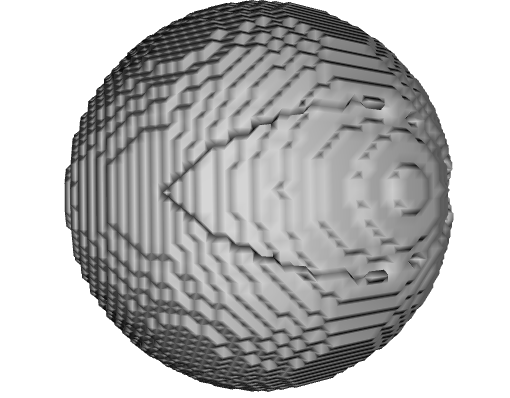
\includegraphics[width=0.4\textwidth]{images/tests/eye03.png}}
  \qquad
  \subfloat[eye\_lr =-0.8, eye\_open = 1.0]{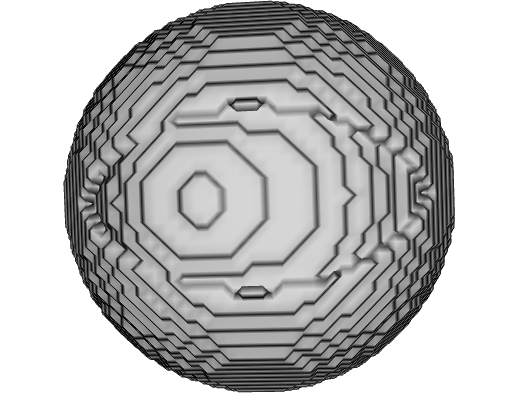
\includegraphics[width=0.4\textwidth]{images/tests/eye04.png}}
  \caption{Wyrenderowane oko cd. (źródło własne).}
\end{figure}

{
\small
\begin{lstlisting}[numbers=left,frame=single,numberstyle=\tiny,backgroundcolor=\color{code_back},breaklines=true]
function abs(x)
  if (x > 0) then
    return x;
  else
    return -x;
  end
end

function eye()
  local pos  = params:getParamFloat("eye_lr");
  local open = params:getParamFloat("eye_open");
  local tmp1 = Sphere();
  local tmp2 = Sphere();
  local tmp3 = Sphere();
  local tmp4 = Sphere();
  local tmp5 = Sphere();

  tmp1:scale(.95,.95,.95);
  tmp2:scale(0.9,0.9,0.9);
  tmp3:scale(1-open*0.2,1-open*0.2, 1-open*0.2);
  tmp3:translate(0,1-open*0.4,0.8);
  tmp4:scale(0.9, 0.9, 0.9);
  tmp5:scale(0.5, 0.5, 0.5);
  tmp5:translate(pos*0.35, 0, 0.92 - abs(pos*0.045));

  local eyelid1 = Diff(tmp1, tmp2, tmp3);
  local eyelid2 = Mirror(eyelid1, 1);

  local eye = Or(eyelid1, eyelid2, tmp4, tmp5);

  return eye;
end
\end{lstlisting}
}

Na początku powyższego kodu znajduje się pomocnicza funkcja {\em abs}, zwraca
ona wartość bezwzględną argumentu. Bezpośrednio pod nią rozpoczyna się funkcja
tworząca oko. Rozpoczyna się ona pobraniem wartości dwóch parametrów zewnętrznych {\em
eye\_lr} i {\em eye\_open}. Dalej znajduje się deklaracja pomocniczych sfer.
Sfery {\em tmp1} - {\em tmp3} stanowią dolną powiekę, natomiast {\em tmp4} i
{\em tmp5} stanowią gałkę oczną i rogówkę. Górną powiekę uzyskaliśmy korzystając
z {\em Mirror} względem płaszczyzny $XZ$.

\subsubsection{Gramatyka nosa}
W przypadku nosa struktura jest już bardziej skomplikowana, jednakże
można uprościć jego budowę do kilku sfer.

\begin{figure}[h!]
  \centering
  \subfloat[Widok z przodu]{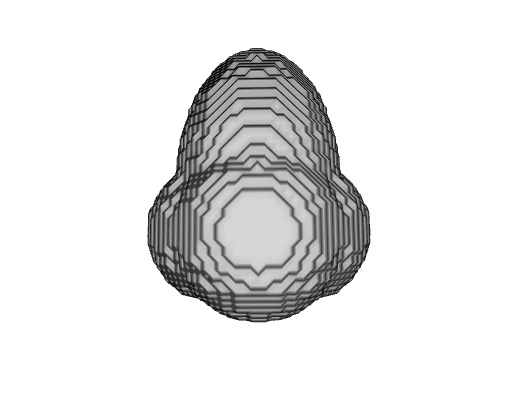
\includegraphics[width=0.4\textwidth]{images/tests/nose01.png}}
  \qquad
  \subfloat[Widok z boku]{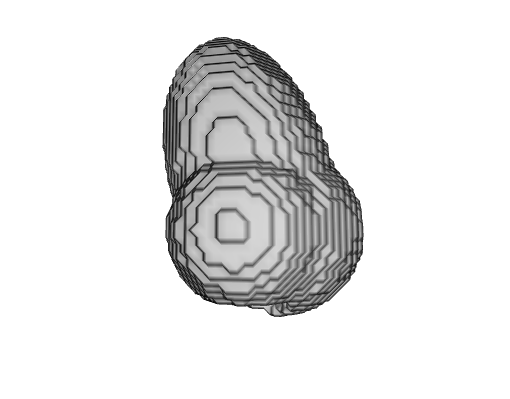
\includegraphics[width=0.4\textwidth]{images/tests/nose02.png}}
  \qquad
  \subfloat[Widok lekko od dołu]{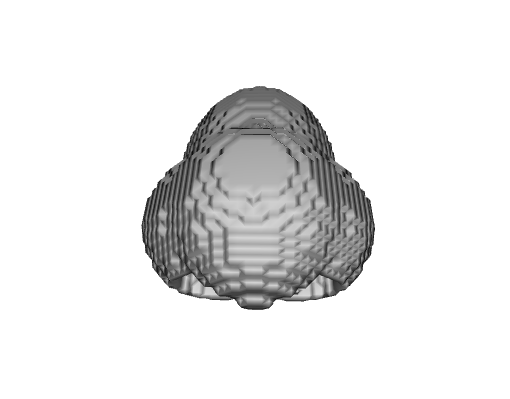
\includegraphics[width=0.4\textwidth]{images/tests/nose03.png}}
  \caption{Wyrenderowany nos (źródło własne).}
\end{figure}

{
\small
\begin{lstlisting}[numbers=left,frame=single,numberstyle=\tiny,backgroundcolor=\color{code_back},breaklines=true]
function nose()
  local bone = Sphere();
  bone:rotate(-0.3, 0, 0);
  bone:scale(0.5, 0.8, 0.5);
  bone:translate(0, 0.2, 0);

  -- czubek
  local tip = Sphere();
  tip:scale(0.45, 0.45, 0.45);
  tip:translate(0, -0.4, 0.25);

  local side1 = Sphere();
  side1:scale(0.4, 0.4, 0.4);
  side1:translate(-0.5, -0.45, -0.05);

  local side2 = Sphere();
  side2:scale(0.4, 0.4, 0.4);
  side2:translate(0.5, -0.45, -0.05);

  local side = Or(side1, side2);

  -- dziurki
  local hole1 = Sphere();
  hole1:scale(0.2, 0.2, 0.2);
  hole1:translate(-1, -2.4, -0.1);

  local hole2 = Sphere();
  hole2:scale(0.2, 0.2, 0.2);
  hole2:translate(1, -2.4, -0.1);

  local holes = Or(hole1, hole2);
  local _nose = Or(bone, tip, side);
        _nose = Diff(_nose, holes);

  return _nose;
end
\end{lstlisting}
}

W liniach 2-5 tworzony jest kształt odpowiadający za górną część nosa (tam gdzie
znajduje się kość), we fragmencie 8-10 tworzony jest kształt, który odpowiada za
czubek nosa. Następnie znajdują się elementy (linie 12-20) tworzące boczne
części nosa -- zewnętrzna część dziurek nosa. Ostatni fragment (linie 23-29)
tworzy kształty, które stanowią dziurki nosa. Na końcu wszystko zostaje
połączone w jeden kształt.

\subsubsection{Gramatyka ust}
Kolejnym częściowym elementem twarzy jaki został poddany modelowaniu są usta. W
tym przypadku model został uproszczony względem rzeczywistego kształtu.

\begin{figure}[h!]
  \centering
  \subfloat[Widok z przodu]{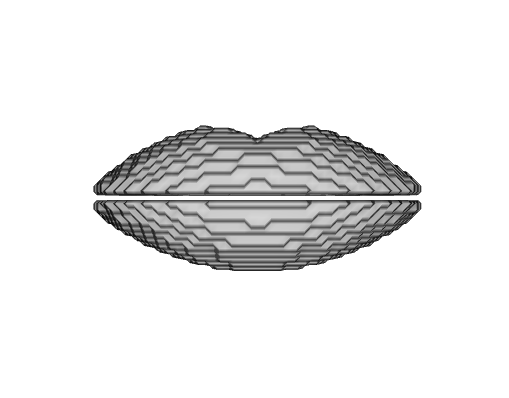
\includegraphics[width=0.4\textwidth]{images/tests/mouth01.png}}
  \qquad
  \subfloat[Widok z boku]{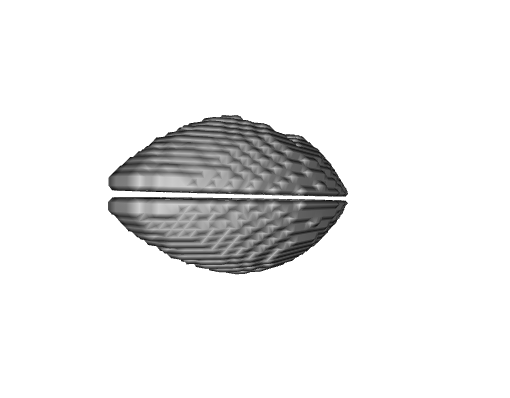
\includegraphics[width=0.4\textwidth]{images/tests/mouth02.png}}
  \caption{Wyrenderowane usta (źródło własne).}
\end{figure}

{
\small
\begin{lstlisting}[numbers=left,frame=single,numberstyle=\tiny,backgroundcolor=\color{code_back},breaklines=true]
function mouth()
  local tmp1 = Sphere();
  local tmp2 = Sphere();
  local tmp3 = Sphere();
  local tmp4 = Sphere();
  local tmp5 = Sphere();
  local tmp6 = Sphere();

  tmp1:scale(1.2, 1, 1);
  tmp1:translate(0, .5, 0);
  tmp2:scale(2.5, 2, 2.5);
  tmp2:translate(0, -1, 0);
  tmp3:scale(1, 0.5, 1);
  tmp3:translate(0, -.55, -.15);
  tmp5:scale(0.8, 0.8, 0.8);
  tmp5:translate(0.4, 0, 0);
  tmp6:scale(0.8, 0.8, 0.8);
  tmp6:translate(-0.4, 0, 0);

  local tmp7 = Diff(tmp4, tmp5, tmp6);
  tmp7:translate(0,-0.42, 0);

  local tmp8 = And(tmp1, tmp2, tmp3);
  tmp8:scale(1, 1, .5);
  tmp8:translate(0, 0.1, 0);

  local tmp9 = Mirror(tmp8, 1);
  tmp9:scale(1, 1.05, 1);

  local tmp10 = Xor(tmp8, tmp9);
  local _mouth = Diff(tmp10, tmp7);
  return _mouth;
end
\end{lstlisting}
}

Sfery {\em tmp1}, {\em tmp2} i {\em tmp3} tworzą kształt wargi dolnej ({\em
tmp8}). Warga górna powstaje jako odbicie lustrzane (modyfikator {\em Mirror} w
linii 27) wargi dolnej oraz wycięcie guzka wargi
górnej\footnote{http://pl.wikipedia.org/wiki/Wargi\_ust} za pomocą sfer {\em
tmp4}, {\em tmp5} i {\em tmp6}, które tworzą element {\em tmp7}.

\subsubsection{Gramatyka ucha}
Ostatnim zamodelowanym elementem twarzy są uszy. Skomplikowana struktura
wymusiła pewne uproszczenia modelu. Model składa się z dwóch części, górnej i
dolnej, które są modelowane osobno a następnie łączone.

\begin{figure}[h!]
  \centering
  \subfloat[Widok z
  przodu]{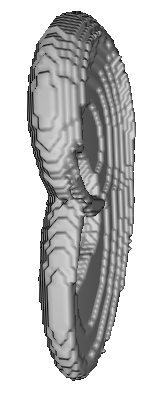
\includegraphics[height=6cm]{images/tests/ear01.png}}
  \qquad
  \subfloat[Widok z
  boku]{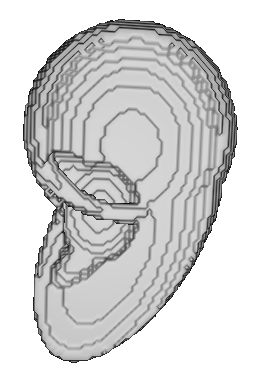
\includegraphics[height=6cm]{images/tests/ear02.png}}
  \caption{Wyrenderowane ucho (źródło własne).}
\end{figure}

{
\small
\begin{lstlisting}[numbers=left,frame=single,numberstyle=\tiny,backgroundcolor=\color{code_back},breaklines=true]
function ear()
  main = Sphere();
  main:scale(0.57, 0.52, 0.2);
  main:translate(0, 0.4, 0);
  
  mainsub = Sphere();
  mainsub:scale(0.8, 0.8, 0.8);
  mainsub:scale(0.57, 0.62, 0.2);
  mainsub:translate(0, 0.33, 0.15);
  
  maind = Sphere();
  maind:scale(0.42, 0.7, 0.2);
  maind:rotateDeg(0, 0, -30);
  maind:translate(0, -0.14, 0);
  
  maindsub = Sphere();
  maindsub:scale(0.42, 0.8, 0.2);
  maindsub:rotateDeg(0, 0, -33);
  maindsub:translate(-0.1, -0.24, 0.2);
  
  hole = Sphere();
  hole:scale(0.22, 0.25, 0.11);
  hole:rotateDeg(0, 0, -11);
  hole:translate(-0.16, 0, 0);
  
  hole1 = Sphere();
  hole1:scale(0.14, 0.25, 0.11);
  hole1:rotateDeg(0, 0, 60);
  hole1:translate(-0.25, 0.12, 0.05);
  hole = Or(hole, hole1);
  
  hole2 = Sphere();
  hole2:scale(0.1, 0.2, 0.11);
  hole2:rotateDeg(0, 0, -50);
  hole2:translate(-0.25, -0.23, 0.05);
  hole = Or(hole, hole2);
  
  maind1 = PlaneProp(maind, 0.5, 0.13);
  maind1:p_rotateDeg(0, 180, 50);
  maind1:p_translate(0.4, -0.6, 0);
  
  edge = Torus(1, 0.12);
  edge:scale(0.5, 0.4, 0.38);
  edge:rotateDeg(93, 0, -4);
  edge:translate(0, 0.38, -0.0);
  
  ear = Or(main, maind1);
  ear = Diff(ear, mainsub);
  ear = Diff(ear, maindsub);
  ear = Diff(ear, hole);
  ear = Or(ear, edge);
  return ear;
end
\end{lstlisting}
}

Sfery {\em main} i {\em mainsub}(wycięcie) tworzą kształt górnej części ucha, a
sfery {\em maind} i {\em maindsub}(wycięcie) kształt dolnej części ucha,
która zostaje dodatkowo wygładzona powierzchnią {\em maind1}. Obiekty {\em
hole}, {\em hole1} i {\em hole2} tworzą wycięcie w uchu. Ostatnim elementem
jest małżowina zamodelowana torusem {\em edge}.

\subsubsection{Struktura głowy}
Ostatnim etapem tworzenia gramatyki twarzy jest ogólna struktura głowy, oraz
odpowiednie umiejscowienie elementów wyżej już przygotowanych. Na początku
utworzona zostanie ogólna struktura gramatyki głowy, a później wszystkie
elementy zostaną połączone w całość.

{
\small
\begin{lstlisting}[numbers=left,frame=single,numberstyle=\tiny,backgroundcolor=\color{code_back},breaklines=true]
function neck()
  local tmp = Cylinder();
  tmp:scale(0.52, 0.7, 0.43);
  tmp:rotateDeg(22, 0, 0);
  local pp = PlaneProp(tmp, 0.5, 0.1);
  pp:p_rotateDeg(0, -90, 0);
  pp:p_translate(0, 0, -0.7);
  return pp;
end

function head_structure()
  local s_skull = Sphere();
  s_skull:scale(0.65, 1.15, 0.76);

  local chin = Torus(1, 0.4);
  chin:scale(0.45, 1, 0.9);
  chin:rotateDeg(45, 0, 0);
  chin:translate(0, 0.2, 0);
  chin:scale(1, 1.3, 0.7);
  local chin_cut = Plane();
  chin_cut:rotateDeg(0, -90, -30);
  chin = Diff(chin, chin_cut);
  s_skull = Or(s_skull, chin);

  --splaszczanie z lewej, prawej
  --od gory, dolu i frontu
  local pl = PlaneProp(s_skull, 0.25, 0.3);
  pl:p_rotateDeg(0, 10, 0);
  pl:p_translate(-0.75, 0, 0);
  local pr = PlaneProp(pl, 0.25, 0.3);
  pr:p_rotateDeg(0, 170, 0);
  pr:p_translate(0.75, 0, 0);
  local pt = PlaneProp(pr, 0.6, 0.4);
  pt:p_rotateDeg(0, 0, -90);
  pt:p_translate(0, 1.1, 0);
  local pb = PlaneProp(pt, 1, 0.25);
  pb:p_rotateDeg(0, 0, 90);
  pb:p_translate(0, -1.2, 0);
  local pf = PlaneProp(pb, 1, 0.2);
  pf:p_rotateDeg(0, 90, -10);
  pf:p_translate(0, 0, 1.2);
  --dodatkowe modelowanie od dolu
  local pb1 = PlaneProp(pf, 0.5, 0.2);
  pb1:p_rotateDeg(30, 0, 90);
  pb1:p_translate(0, -1.2, 0);
  local pl1 = PlaneProp(pb1, 0.5, 0.12);
  pl1:p_rotateDeg(0, 20, 30);
  pl1:p_translate(-0.6, -0.5, 0.55);
  local pr1 = PlaneProp(pl1, 0.5, 0.1);
  pr1:p_rotateDeg(0, 160, 30);
  pr1:p_translate(0.6, -0.5, 0.6);

  --wglebienie na oczy
  local eyes = Torus(2, 0.3);
  eyes:scale(0.44, 0.56, 0.49);
  eyes:translate(0, 0.07, -0.29);
  --wyciecie z wglebienia, bez srodka
  local e1 = Sphere();
  e1:scale(0.5, 0.5, 0.5);
  e1:translate(0.52, 0.1, 0.7);
  local e2 = Sphere();
  e2:scale(0.5, 0.5, 0.5);
  e2:translate(-0.52, 0.1, 0.7);

  local tc = Cube()
  tc:scale(1, 0.23, 0.3);
  tc:translate(0, 0.08, 0.29);
  tc1 = Diff(tc, e1);
  tc2 = Diff(tc1, e2);

  local faced = Sphere()
  faced:scale(0.6, 1, 0.65)
  faced:translate(0, -0.3, 0.04);
  local fp = PlaneProp(faced, 0.6, 0.4);
  fp:p_rotateDeg(0, 90, 0);
  fp:p_translate(0, 0, 1);
  local c = Cube();
  c:scale(0.58, 0.6, 0.3);
  c:translate(0, -0.55, 0.45);
  local cutOut = Diff(And(pr1, c), fp)
  local all = Diff(pr1, cutOut);

  eyes1 = Diff(eyes, tc2);
  all = Diff(all, eyes1);
  return all;
end
\end{lstlisting}
}
Struktura głowy została podzielona na dwie logiczne części: czaszkę i
szyję. Pierwsza funkcja {\em neck} (linie 1-12) tworzy kształt bazujący na
cylindrze, który będzie szyją. Druga funkcja {\em head\_structure}
przygotowuje ogólny model głowy. W linii 11 tworzona jest sfera reprezentująca
głowę, a następnie do elementu dodawany jest podbródek (linie 14-22).
Kolejnym krokiem jest odpowiednie wymodelowanie kształtu głowy (linie 26-50).
W liniach 53-83 modelowany jest element tworzący oczodoły i zostaje odjęty od
aktualnego kształtu głowy.
Połączone elementy zaprezentowane są na ilustracjach~\ref{skull}.

\begin{figure}[h!]
  \centering
  \subfloat[Widok z przodu]{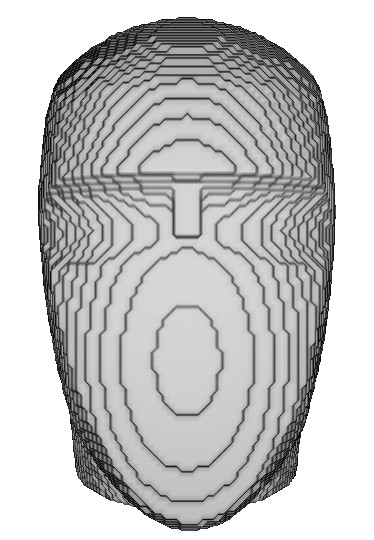
\includegraphics[width=0.4\textwidth]{images/tests/skull01.png}}
  \qquad
  \subfloat[Widok z boku]{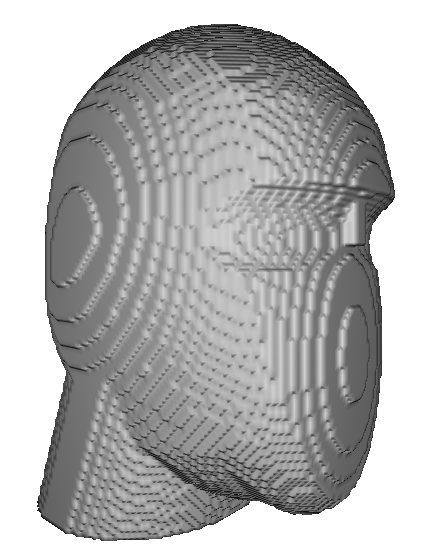
\includegraphics[width=0.4\textwidth]{images/tests/skull02.png}}
  \caption{Wyrenderowana głowa bez oczu, nosa i ust (źródło własne).}
  \label{skull}
\end{figure}

Ostatnim elementem jest połączenie wszystkiego w jedną całość oraz
sparametryzowanie wielkości i położenia nosa, oczu i ust.

\begin{figure}[h!]
  \centering
  \subfloat[Widok z
  przodu]{\label{fig:final_head1}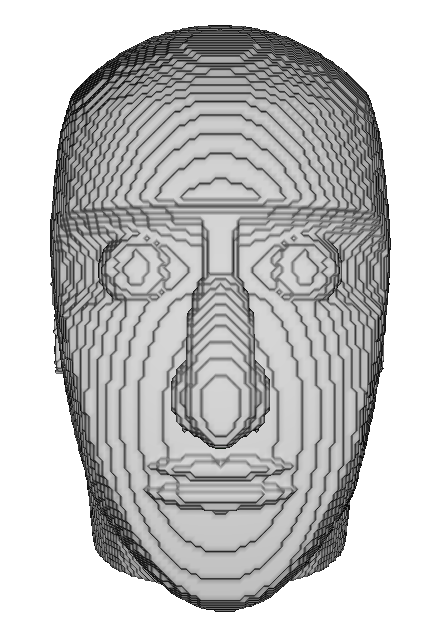
\includegraphics[height=7cm]{images/tests/head01.png}}
  \qquad
  \subfloat[Widok z
  boku]{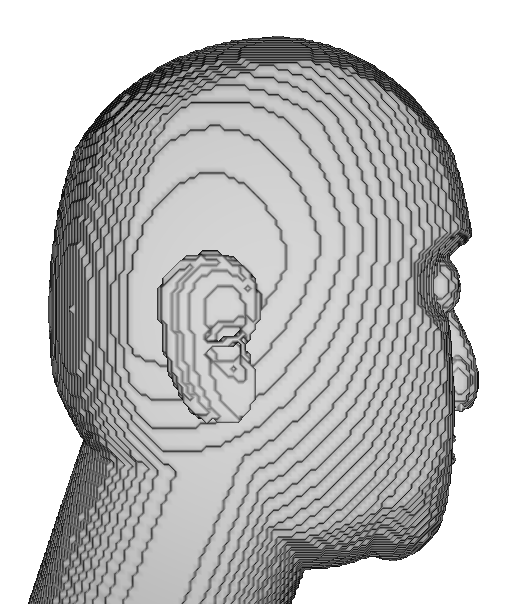
\includegraphics[height=7cm]{images/tests/head02.png}\label{fig:final_head2}}
  \qquad
  \subfloat[Widok z pod kątem
  30$^o$]{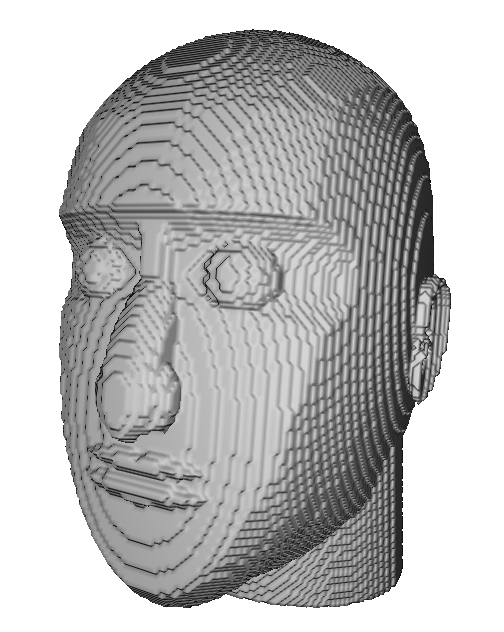
\includegraphics[height=7cm]{images/tests/head03.png}\label{fig:final_head3}}
  \qquad
  \subfloat[Dodatkowy
  widok]{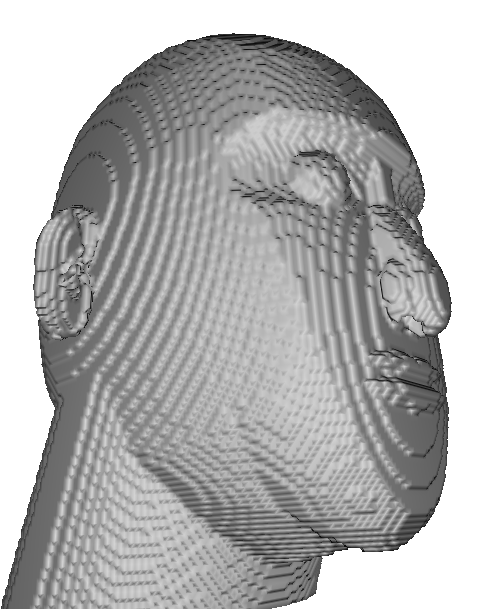
\includegraphics[height=7cm]{images/tests/head04.png}\label{fig:final_head4}}
  \caption{Wyrenderowana głowa (źródło własne).}
  \label{fig:final_head}
\end{figure}

{
\small
\begin{lstlisting}[numbers=left,frame=single,numberstyle=\tiny,backgroundcolor=\color{code_back},breaklines=true]
local nose_sx = params:getParamFloat("nose_sx");
local nose_sy = params:getParamFloat("nose_sy");
local nose_sz = params:getParamFloat("nose_sz");
local nose_ty = params:getParamFloat("nose_ty");
local nose_tz = params:getParamFloat("nose_tz");

local eye_scale = params:getParamFloat("eye_scale");
local eye_tx = params:getParamFloat("eye_tx");
local eye_ty = params:getParamFloat("eye_ty");
local eye_tz = params:getParamFloat("eye_tz");

local mouth_sx = params:getParamFloat("mouth_sx");
local mouth_sy = params:getParamFloat("mouth_sy");
local mouth_sz = params:getParamFloat("mouth_sz");
local mouth_ty = params:getParamFloat("mouth_ty");
local mouth_tz = params:getParamFloat("mouth_tz");

local HeadStructure = head_structure();
local Neck = neck();
Neck:translate(0, -1.0, -0.42);
local EarR = ear();
local earSize = 0.25;
EarR:scale(earSize, earSize, earSize);
EarR:rotateDeg(0, 80, 0);
EarR:translate(0.6, -0.09, -0.17);
local EarL = Mirror(EarR, 0);

local Nose = nose();
Nose:translate(0, nose_ty, nose_tz);
Nose:scale(nose_sx, nose_sy, nose_sz);

local Mouth = mouth();
Mouth:translate(0, mouth_ty, mouth_tz);
Mouth:scale(mouth_sx, mouth_sy, mouth_sz);

local EyeL = eye();
EyeL:translate(eye_tx, eye_ty, eye_tz);
EyeL:scale(eye_scale, eye_scale, eye_scale);
local EyeR = Mirror(EyeL, 0);

local Head = Or(Neck, HeadStructure);
Head = Or(Head, EarR);
Head = Or(Head, EarL);
Head = Or(Head, Nose);
Head = Or(Head, Mouth);
Head = Or(Head, EyeL);
Head = Or(Head, EyeR);
draw(Head);
\end{lstlisting}
}

W liniach 1-16 pobierane zostają parametry określające odpowiednio wielkość i
położenie nosa, wielkość i położenie oczu i wielkość i położenie ust. Następnie
w liniach 18-26 wygenerowane zostają kolejne elementy głowy: ogólna struktura
(18), szyja (19), prawe ucho (21) oraz, przy użyciu operacji \emph{Mirror}, lewe
ucho (26). W dalszej kolejności utworzone i sparametryzowane są: nos (28-30),
usta (32-34), prawe i lewe oko (36-39). W liniach 41-47 wszystkie
elementy zostają połączone, po czym zostają wyświetlone na ekranie (linia 40).
Ilustracje~\ref{fig:final_head1},~\ref{fig:final_head2},~\ref{fig:final_head3},~\ref{fig:final_head4}
przedstawiają wygenerowaną głowę.
